\newpage
\section{TIRISTORES TRIAC}
\sangria{Para la actividad 5, se analizó el comportamiento de un TRIAC BT137 controlado por un DIAC en su compuerta, según el esquema de la figura 14,donde se fijaron distintas tensiones de alimentación $V_{CC}$ (80V, 130V, etc.) y se midió la corriente de ánodo ($I_A$) en función de la corriente de compuerta ($I_G$).}
\sangria{El análisis de dichas mediciones revela los tres estados fundamentales del TRIAC:
Primero, se comprueba el \textbf{estado de bloqueo}. Con $V_{CC} = 100V$ aplicados, una corriente de compuerta $I_G = 523.3 \mu A$ (generada por $V_G = 15V$) es insuficiente para activar el dispositivo, resultando en una corriente de ánodo $I_A = 0$.
Segundo, se identifica el \textbf{disparo}. Las notas indican un punto de disparo claro donde se requiere una corriente de compuerta $I_{GT} \approx 3.4 mA$ (con $V_G = 3.2V$) para que el TRIAC se encienda y permita el flujo de una corriente de carga $I_A = 37.6 mA$. Esto demuestra la función de control del dispositivo: una pequeña corriente de compuerta conmuta una corriente de carga mucho mayor.
Finalmente, y de manera crucial, las mediciones demuestran el \textbf{efecto de enganche (latching)}. Se registra un punto donde, tras el disparo, la corriente de compuerta se reduce a $I_G = 0 mA$ (con $V_G$ residual de 0.7V), pero el TRIAC \textbf{permanece encendido}, sosteniendo una corriente de carga $I_A = 16.3 mA$. Este fenómeno es la característica principal de un tiristor: una vez activado, ya no necesita la señal de disparo para seguir conduciendo. El dispositivo solo se apagará si la corriente de carga $I_A$ cae por debajo de la \textbf{corriente de mantenimiento ($I_H$)}.}


\begin{center}
\small
\setlength{\tabcolsep}{4pt}
\captionof{table}{Valores del TRIAC relevados en el laboratorio.}
\begin{tabular}{|
>{\columncolor[HTML]{FFCCC9}}l |
l | l |
l | l | l |
l | l | l |}
\hline


\rowcolor[HTML]{FFFFC7}
& \multicolumn{2}{c|}{\textbf{$V_i = 80V$}}
& \multicolumn{3}{c|}{\textbf{$V_i = 130V$}}
& \multicolumn{3}{c|}{\textbf{$V_i = 180V$}} \\


\rowcolor[HTML]{FFFFC7}
\textbf{$V_G$ [V]}
& \textbf{$I_G$ [mA]} & \textbf{$I_A$ [mA]}
& \textbf{$V_G$ [V]} & \textbf{$I_G$ [mA]} & \textbf{$I_A$ [mA]}
& \textbf{$V_G$ [V]} & \textbf{$I_G$ [mA]} & \textbf{$I_A$ [mA]} \\ \hline


0 & 0 & 0 & 0 & 0 & 0 & 0 & 0 & 0 \\ \hline
10 & 0 & 0 & 10 & 0 & 0 & 10 & 0 & 0 \\ \hline
20 & 0 & 0 & 20 & 0 & 0 & 20 & 0 & 0 \\ \hline
30 & 0 & 0 & 30 & 0 & 0 & 30 & 0 & 0 \\ \hline
31 & 0 & 0 & 31 & 0 & 0 & 32 & 0 & 31.7 \\ \hline
32 & 3.4 & 3.4 & 31.6 & 4.53 & 4.57 & --- & --- & --- \\ \hline
23.3 & 3.8 & 3.9 & 28.4 & 4.53 & 4.53 & --- & --- & --- \\ \hline
23.1 & 4.15 & 4.15 & 0.3 & 0 & 26.7 & --- & --- & --- \\ \hline
23.2 & 4.6 & 4.8 & --- & --- & --- & --- & --- & --- \\ \hline
23.2 & 4.3 & 6 & --- & --- & --- & --- & --- & --- \\ \hline
23.3 & 4.1 & 6.2 & --- & --- & --- & --- & --- & --- \\ \hline
0.7 & 0 & 16.3 & --- & --- & --- & --- & --- & --- \\ \hline
\end{tabular}
\end{center}

\begin{figure}[H]
    \centering
    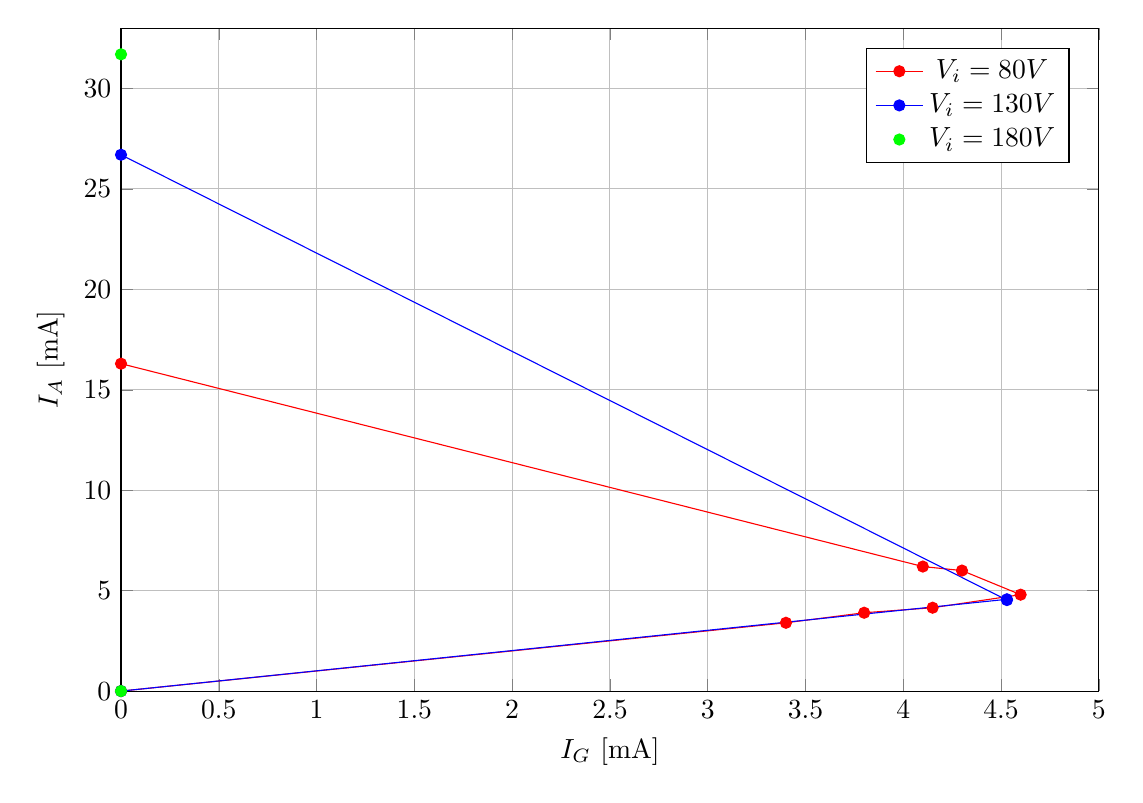
\begin{tikzpicture}
        \begin{axis}[
            width=14cm, % Ancho del gráfico
            height=10cm, % Alto del gráfico
            xlabel={$I_G$ [\si{mA}]}, % Eje X
            ylabel={$I_A$ [\si{mA}]}, % Eje Y
            legend pos=north east,
            grid=major,
            xmin=0, xmax=5,
            ymin=0, ymax=33,
        ]
        \addplot [
            color=red,
            mark=*,
            mark size=2pt,
        ]
        coordinates {
            (0, 0)
            (3.4, 3.4)
            (3.8, 3.9)
            (4.15, 4.15)
            (4.6, 4.8)
            (4.3, 6)
            (4.1, 6.2)
            (0, 16.3)
        };
        \addlegendentry{$V_i = 80V$}
        \addplot [
            color=blue,
            mark=*,
            mark size=2pt,
        ]
        coordinates {
            (0, 0)
            (4.53, 4.57)
            (4.53, 4.53)
            (0, 26.7)
        };
        \addlegendentry{$V_i = 130V$}
        \addplot [
            color=green,
            only marks,
            mark=*,
            mark size=2pt,
        ]
        coordinates {
            (0, 0)
            (0, 31.7)
        };
        \addlegendentry{$V_i = 180V$}

        \end{axis}
    \end{tikzpicture}
    \caption{Familia de curvas experimentales $I_A = f(I_G)$ para distintos valores de $V_i$}
\end{figure}

\subsection{Conclusiones}
\sangria{Nos pareció raro comparar $I_G$ con $I_A$, pero podemos ver que para una mayor $VCC$ aumentamos el valor de disparo en la tensión $V_G$, la curva nos queda aceptable, pero para $VCC = 180V$, el disparo ocurre demasiado rapido y no pudimos medir la curva correctamente}

\midTitle{blue}{Notas del documentador:}{TRIAC}
\sangria{Tuvimos incovenientes para hacer disparar el triac en 180$V$, solamente pudimos medir después del disparo la $I_A$}

\section{Dimmer y controlador de potencia}

\sangria{En esta actividad final se analiza la aplicación más común de los tiristores: el control de potencia en corriente alterna (CA) mediante un circuito "dimmer". El objetivo es observar el funcionamiento del TRIAC en un circuito real alimentado por la red eléctrica. El circuito, detallado en la Figura 15, utiliza un TRIAC (TIC 226) como interruptor principal en serie con la carga. El control de este interruptor se logra mediante una red de disparo compuesta por un DIAC, un capacitor, y una resistencia variable (potenciómetro) de 250K. El principio de funcionamiento es el \textbf{control de ángulo de fase}. En cada semiciclo de la onda de CA de entrada, el capacitor se carga a través del potenciómetro. La velocidad de esta carga es determinada por la constante de tiempo RC, la cual se ajusta variando la resistencia del potenciómetro. Cuando la tensión acumulada en el capacitor alcanza la tensión de ruptura ($V_{BO}$) del DIAC (indicada como 30V en el diagrama), el DIAC se dispara. Al dispararse, actúa como un interruptor cerrado y descarga abruptamente el capacitor sobre la compuerta (Gate) del TRIAC.}
\sangria{El pulso de corriente ($I_G$) dispara al TRIAC, poniéndolo en estado de conducción. Una vez encendido, el TRIAC permite que la corriente fluya hacia la carga durante el \textbf{resto} de ese semiciclo. Cuando la onda de CA cruza por cero, la corriente que atraviesa el TRIAC cae por debajo de su corriente de mantenimiento ($I_H$), provocando su \textbf{apagado natural} (conmutación natural). El proceso se repite idénticamente en el siguiente semiciclo, pero con polaridad opuesta, gracias a la naturaleza bidireccional del DIAC y el TRIAC.}

\sangria{El efecto de "dimmer" (atenuación) se logra al variar el potenciómetro:
\begin{itemize}
    \item \textbf{Resistencia alta:} El capacitor tarda más en cargarse. El disparo del TRIAC ocurre tarde en el semiciclo. Se entrega poca potencia a la carga (luz tenue).
    \item \textbf{Resistencia baja:} El capacitor se carga rápidamente. El disparo del TRIAC ocurre temprano en el semiciclo. Se entrega mucha potencia a la carga (luz intensa).
\end{itemize}
De esta forma, el circuito controla la potencia transferida a la carga ajustando el ángulo de fase en el que comienza la conducción.}
\imagen[Disparo del triac con la menor resistencia]{15cm}{./imagenes/triac1.jpg}
\imagen[Disparo del triac con una resistencia media]{15cm}{./imagenes/triac2.jpg}
\imagen[Disparo del triac con la mayor resistencia]{15cm}{./imagenes/triac3.jpg}

\midTitle{blue}{Notas del documentador:}{Dimmer}
\sangria{En esta experiencia tuvimos problemas con la red eléctrica, ya que quemamos 2 puntas de osciloscopio e hicimos saltar la térmica del banco de trabajo, pero si logramos medir correctamente la experiencia}

